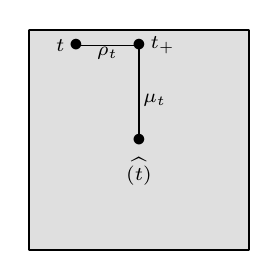
\begin{tikzpicture}[auto, scale = 2]
      \draw [fill = gray!25, draw = gray!75] (0,0) rectangle (1.4,1.4);
      \draw [thick] (0,0) -- (1.4,0);
      \draw [thick] (0,0) -- (0,1.4);
      \draw [thick] (1.4,0) -- (1.4,1.4);
      \draw [thick] (0,1.4) -- (1.4,1.4);
      \node (s-) at (0.7,1.3) {$\bullet$};
      \node at (0.85,1.3) {\scriptsize{$t_+$}};
      \node (s) at (0.3,1.3) {$\bullet$};
      \node at (0.2,1.3) {\scriptsize{$t$}};
      \node (hs) at (0.7,0.7) {$\bullet$};
      \node at (0.7,0.5) {\scriptsize{$\widehat {\carrier(t)}$}};
      \draw (0.7,1.3) -- (0.7,0.7);
      \draw (0.7,1.3) -- (0.3,1.3);
      \node at (0.8,0.95) {\scriptsize{$\mu_t$}};
      \node at (0.5,1.25) {\scriptsize{$\rho_t$}};
    \end{tikzpicture}
    \qquad\qquad
    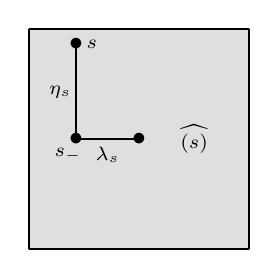
\begin{tikzpicture}[auto,scale = 2]
      \draw [fill = gray!25, draw = gray!75] (0,0) rectangle (1.4,1.4);
      \draw [thick] (0,0) -- (1.4,0);
      \draw [thick] (0,0) -- (0,1.4);
      \draw [thick] (1.4,0) -- (1.4,1.4);
      \draw [thick] (0,1.4) -- (1.4,1.4);
      \node (s-) at (0.3,0.7) {$\bullet$};
      \node at (0.25,0.6) {\scriptsize{$s_-$}};
      \node (s) at (0.3,1.3) {$\bullet$};
      \node at (0.4,1.3) {\scriptsize{$s$}};
      \node (hs) at (0.7,0.7) {$\bullet$};
      \node at (1.05,0.7) {\scriptsize{$\widehat {\carrier(s)}$}};
      \draw (0.3,0.7) -- (0.7,0.7);
      \draw (0.3,0.7) -- (0.3,1.3);
      \node at (0.5,0.6) {\scriptsize{$\lambda_s$}};
      \node at (0.2,1.0) {\scriptsize{$\eta_s$}};
    \end{tikzpicture}